\documentclass[a4paper]{extreport}
\usepackage[italian,english]{babel}
\bibliographystyle{alpha}
\title{\Huge Studio Esecutivo}
\usepackage{geometry,subcaption,float}
\usepackage[plainpages=false,
colorlinks=ture,
linkcolor= blue,
urlcolor = blue,
citecolor = green,
anchorcolor = blue]{hyperref}
\geometry{a4paper, top=3cm, bottom=3cm, left=3.5cm, right=3.5cm, heightrounded, bindingoffset=5mm}
\author{Luca Rossicone, Filippo Iacobelli}
\begin{document}
\selectlanguage{italian}
\maketitle
\large
\section*{Julia Artifacts}
Gli artefatti\cite{artifacts} in Julia esistono sotto forma di un modulo all'interno del modulo Pkg chiamato Pkg.Artifacts. Si accede alla funzionalità nel REPL tramite:
\begin{verbatim}
    julia> using Pkg.Artifacts    
\end{verbatim}
Se inserire immagini, file binari, set di dati e dati simili nei repository git fosse indolore e senza problemi, potremmo non aver bisogno di Artifacts.\\
Il problema è che per i file binari i requisiti di spazio possono diventare eccessivi abbastanza rapidamente.
Compilare una versione per ogni piattaforma, 32-bit, 64-bit e una moltitudine di altre varianti e mantenerla nella libreria del codice sorgente è una pratica troppo onerosa: ci vorrebbe troppo spazio.\\
Con Artifacts, più pacchetti potrebbero in linea di principio utilizzare gli stessi dati e non è necessario scaricarli due volte. Facciamo conto che il pacchetto A e il pacchetto B, entrambi dipendono dalla libreria Qt. La soluzione fittizia a questo è che entrambe le librerie memorizzino una copia di Qt.\\
Bisognerebbe quindi scaricare un'enorme libreria due volte sprecando il doppio dello spazio sul disco rigido. Non è una buona soluzione. Ora qualcun altro potrebbe pensare di essere intelligente e archiviare Qt in una directory condivisa per entrambi i pacchetti da usare. Vari sistemi operativi lo hanno fatto all'inizio e hanno creato la cosa divertente che chiamiamo "inferno DLL". Ciò accade quando la versione Qt richiesta non è proprio la stessa. La versione scaricabile Qt potrebbe funzionare per A, ma non per B.\\
Git ha reso popolare una soluzione a questo enigma chiamato dati indirizzabili al contenuto. Ciò significa che non localizzano i dati fornendo percorsi come \verb|A/libs/Qt|, ma usiamo invece degli hash.\\
In questo caso, ogni byte dei binari della libreria Qt viene inserito in un algoritmo di hashing e crea un numero univoco, l'hash. In teoria, ovviamente, non è possibile garantire che due set di dati producano hash diversi. La possibilità che diversi set di dati producano lo stesso hash è simile a quella di due persone in posizioni casuali sulla terra che raccolgono lo stesso granello di sabbia. Potrebbe succedere, ma è improbabile.\\
Il sistema di pacchetti Julia può quindi verificare se una libreria è stata già installata controllando se esiste già una directory con un hash ed evitare di scaricare la stessa libreria una seconda volta.
\\Un altro problema risolto con Artifacts è che si evita di gonfiare il proprio repository con file binari. Supponiamo che tu abbia un pacchetto \verb|Museo| con il codice per mostrare i \verb|quadri|. Invece di inserire una directory \verb|quadri| nel repository del pacchetto con le immagini di ogni opera d'arte, crei un file \verb|Artifacts.toml|. In esso descrivi dove si trovano le varie immagini in una maniera simile a questa
{\small\begin{verbatim}
    # Museo/Artifacts.toml 
    [pictures]
    git-tree-sha1 = "c5f4d31e5c9c5d6fba2469ceff3d9916050d92d2"
    lazy = true

    [[pictures.download]]
    sha256 = "2aea399ab3c6b6e3a4285ec6ae31b858803442bf1b3e3e4889a2e3e8287d56c6"
    url = "https://github.com/johndoe/Museo.jl/releases/download/pictures.tar.gz"
\end{verbatim}}
\section*{Thread}
Un thread è un singolo flusso sequenziale di controllo all'interno di un programma.~\cite{threads}\\
La vera eccitazione che circonda i thread non riguarda un singolo thread sequenziale. Piuttosto, si tratta dell'uso di più thread in esecuzione contemporaneamente ed eseguire attività diverse in un unico programma. Questo uso è illustrato nella figura successiva.
% \begin{figure}[!ht]
%     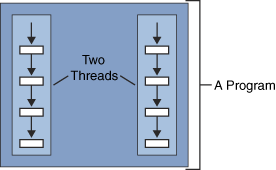
\includegraphics[width=\linewidth]{immagini/threads-two.png}
% \end{figure}
\\Un browser Web è un esempio di applicazione multithread. All'interno di un browser tipico, puoi scorrere una pagina mentre sta scaricando un'applet o un'immagine, riprodurre animazioni e suoni contemporaneamente, stampare una pagina in background mentre scarichi una nuova pagina o guardare tre algoritmi di ordinamento che corrono verso il traguardo.
\\Alcuni testi chiamano un thread un processo leggero. Un thread è simile a un processo reale in quanto entrambi hanno un unico flusso sequenziale di controllo. Tuttavia, un thread è considerato leggero perché viene eseguito nel contesto di un programma completo e sfrutta le risorse allocate per quel programma e l'ambiente del programma.
\section*{Tasks}
Una coroutine o task è simile a un thread: è una linea di esecuzione, con il proprio stack, le proprie variabili locali e il proprio
puntatore alle istruzioni; il tutto però è condiviso con altre coroutine. La principale differenza tra thread e coroutine è che,
concettualmente (o letteralmente, in una macchina multiprocessore), un programma con thread esegue diversi thread in parallelo. 
Le coroutine, d'altra parte, sono collaborative: in un dato momento, un programma con coroutine esegue solo una delle sue coroutine
e questa coroutine in esecuzione sospende la sua esecuzione solo quando richiede esplicitamente di essere sospesa.~\cite{tasks}\\
L'istruzione 'yield' in Julia ha lo scopo di creare coroutine. Quando si incontra l'istruzione 'yield', lo stato corrente della
funzione viene salvato e il controllo viene restituito alla funzione chiamante.
La funzione chiamante può quindi ritrasferire l'esecuzione alla funzione cedente e il suo stato verrà ripristinato al punto in cui
è stato riscontrato lo 'yield' e l'esecuzione continuerà.
\bibliography{sitografia}
\end{document}